%!TEX root = ../../Main.tex
\graphicspath{{Chapters/Indledning/}}
%-------------------------------------------------------------------------------

\section{Indledning}
Næsten alle danskere har nu til dags en smartphone med indbygget bluetooth modul, som man altid har med på sig når man forlader sit hjem. Dette vil vi gerne udnytte til at kunne gøre det nemmere for brugere, at kunne låse op og låse hoveddøren, som adskiller omverdenen fra ens dyrebare ejendele. Dette betyder at forbrugeren aldrig skal tænke mere på nøgler, da disse bliver overflødige. Dermed slipper brugeren for at skulle huske på dette, samt at skulle fumle med nøglerne når man kommer hjem med flere poser i hænderne fra dagens indkøbstur. 

Denne prototype, BA-TA (Bluetooth Anti-Theft Alarm), vil derfor hhv. kunne låse op og låse hoveddøren, så snart systemet registrerer at husets ejer og dermed ejerens smartphone er i nærheden eller ej.


Hele systemet styres fra en samlet enhed, som kan integeres fra brugeren gennem en skærm og dertilhørende touch funktion. 

\begin{figure}[H]
	\centering
	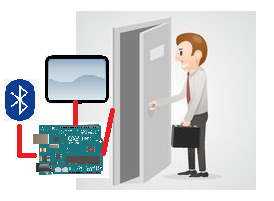
\includegraphics[width = 300 pt]{Img/Konceptbillede.png}
	\caption{Konceptbillede}
	\label{fig:Konceptbillede}
\end{figure}

Igennem brugergrænsefladen kan brugeren tilføje og fjerne enheder (personer) som skal kunne låse og låse op for døren.

Når alle godkendte enheder er uden for rækkevidde af systemets bluetooth scanner, låses døren, og så snart systemet ser en godkendt enhed indenfor rækkevidden bliver døren låst op. 

